% Options for packages loaded elsewhere
\PassOptionsToPackage{unicode}{hyperref}
\PassOptionsToPackage{hyphens}{url}
\documentclass[
  12pt,
  ignorenonframetext,
  aspectratio=169,
  french,
  aspectratio=169]{beamer}

%%%%%%%%%%%%%%%%%%%%%%%%%%%%%%%%%%%%%%%%%%%%%%%%%%%%%%%%%%%%%%%%%%%%%%%%%%%%%%
% \embedvideo{<poster or text>}{<video file (MP4+H264)>}
% \embedvideo*{...}{...}                     % auto-play
%%%%%%%%%%%%%%%%%%%%%%%%%%%%%%%%%%%%%%%%%%%%%%%%%%%%%%%%%%%%%%%%%%%%%%%%%%%%%%
\usepackage[bigfiles]{pdfbase}
\usepackage{xkeyval}
\makeatletter
\define@boolkey{simplemedia}{autoplay}{\def\simplemediaautoplay{#1}}
\define@boolkey{simplemedia}{showGUI}{\def\simplemediashowGUI{#1}}
\presetkeys{simplemedia}{autoplay=true,showGUI=true}{}

% all page-references relate to: Adobe PDF Reference, sixth edition, November 2006, can be found e.g.:
%https://ghostscript.com/~robin/pdf_reference17.pdf
%%%%%%%%%%%%%%%%%%%%%%%%%%%%%%%%%%%%%%%%%%%%%%%%%%%%%%%%%%%%%%%%%%%%%%%%%%%%%%
% \simplemedia[<options>]{<poster or text>}{<media file>}{MIME type}
%%%%%%%%%%%%%%%%%%%%%%%%%%%%%%%%%%%%%%%%%%%%%%%%%%%%%%%%%%%%%%%%%%%%%%%%%%%%%%
\ExplSyntaxOn
%\cs_new:Npn\simplemedia[3][]{
\newcommand\simplemedia[4][]{%
  \setkeys{simplemedia}{#1}%
  \leavevmode
  \pbs_pdfobj:nnn{}{fstream}{{}{#3}}
  \pbs_pdfobj:nnn{}{dict}{
    /Type/Filespec/F~(#3)/UF~(#3)
    /EF~<</F~\pbs_pdflastobj:>>
  }
  %
  \pbs_pdfobj:nnn{}{dict}{
      /CT~(#4)% content type, page 764, table 9.9
      /D~\pbs_pdflastobj:% full file spcification, page 764, table 9.9
      /N~(Media~clip~from~#3)% name of media clip, page 764, table 9.8
      /P~<</TF (TEMPACCESS)>>% media permissions, page 764, table 9.9
      /S~/MCD% subtype media-clip-data, page 764, table 9.8
  }
  %
  \pbs_pdfobj:nnn{}{dict}{
      /C~\pbs_pdflastobj:% media clip dictionary, page 762, table 9.6
      /N~(RenditionFrom#3)% name of rendition, page 759, table 9.1
      /P~<<% media play parameters dictionary, page 762, table 9.6
%%%%%%%%%%%%%%%%%%%%%%%%%%%%%%%%%%%%%%%%%%%%%%%%%%%%%%%%%%%%%%%%%%%%%%%%%%%%%%%%%%%%%%%%%%%%%%%%%%%%%%%%%%%%%%%%%%%%%%%%%%
%       Here's the point to switch on/off player GUI
%%%%%%%%%%%%%%%%%%%%%%%%%%%%%%%%%%%%%%%%%%%%%%%%%%%%%%%%%%%%%%%%%%%%%%%%%%%%%%%%%%%%%%%%%%%%%%%%%%%%%%%%%%%%%%%%%%%%%%%%%%
        /BE~<</C~\simplemediashowGUI~%C: display a player-specific controller user interface, page 769, table 9.15
        /A~true>>~%A: automatically play when activated, page 770, table 9.15
        % select player (not used here)
%        /PL~<</A~[% arrray of media player info objects page 777
%%        <</PID~<</U~(vnd.adobe.swname:ADBE_MCI)~>>~>>~% PID: software identifier object, page 779
%        <</PID~<</U~(vnd.adobe.swname:MSFT_WindowsMediaPlayer)~/OS[(win16)~(win32)~(win9x)~(winnt)~(wince)]>>~>>~%/OS operating system, page 780
%        ]~>>
      ~>>
      /S~/MR% subtype of rendition, page 759, table 9.1
  }
  %
  \tl_set:Nx\mediarendition{\pbs_pdflastobj:}
  %  
  \pbs_pdfobj:nnn{}{dict}{}% obj-number created for later use
  \tl_set:Nx\renditionactionplay{\pbs_pdflastobj:}%
  %
  \pbs_pdfobj:nnn{}{dict}{}% obj-number created for later use
  \tl_set:Nx\renditionactionstop{\pbs_pdflastobj:}%
  %
  \hbox_set:Nn\l_tmpa_box{#2}% size of annotation
  \tl_set:Nx\l_box_wd_tl{\dim_use:N\box_wd:N\l_tmpa_box}
  \tl_set:Nx\l_box_ht_tl{\dim_use:N\box_ht:N\l_tmpa_box}
  \tl_set:Nx\l_box_dp_tl{\dim_use:N\box_dp:N\l_tmpa_box}
  \pbs_pdfxform:nnnnn{1}{1}{}{}{\l_tmpa_box}
  %
  \tl_set:Nx\l_simplem_current_page_tl{\zref@extract{simplem@\int_use:N\g_simplem_id_int}{abspage}}
  \pbs_pdfannot:nnnn{\l_box_wd_tl}{\l_box_ht_tl}{\l_box_dp_tl}{
      /T~(AnnotationFrom#3)~% title of screen annotation, page 640, table 8.38 
      /Subtype~/Screen~% Subtype Sreen, page 616, table 8.20 and page 640, table 8.38
      /BS~<</W~1/S/S>>% Borderstyle
      /C~[0.039216~0.039216~0.039216]% color used background, title bar, border, page 607, table 8.15
      /Contents~(EmbeddedAudiofile#3)% Text to be displayed, page 606, table 8.15
      /NM~(audioscreenannot:#3)% annotation name, page 606, table 8.15
      /AP~<</N~\pbs_pdflastxform:>>% appearance dictionary, page 606, table 8.15
      /F~4~%Annotation flag, page 606, table 8.15 and page 608, table 8.16
      /A~\renditionactionplay~% Action to be performed, page 640 
%%%%%%%%%%%%%%%%%%%%%%%%%%%%%%%%%%%%%%%%%%%%%%%%%%%%%%%%%%%%%%%%%%%%%%%%%%%%%%%%%%%%%%%%%%%%%%%%%%%%%%%%%%%%%%%%%%%%%%%%%%
%       Here's the point to switch on/off autoplay
%%%%%%%%%%%%%%%%%%%%%%%%%%%%%%%%%%%%%%%%%%%%%%%%%%%%%%%%%%%%%%%%%%%%%%%%%%%%%%%%%%%%%%%%%%%%%%%%%%%%%%%%%%%%%%%%%%%%%%%%%%
      % autoplay is realised by "additional action" (page 640), 
      % PageOpen (PO) -> play "Play Rendition"
      % PageClose (PC) -> play "Stop Rendition" (see page 650)
      /AA~<<\ifKV@simplemedia@autoplay~/PO~\renditionactionplay~\fi~/PC~\renditionactionstop~>>~%
%%%%%%%%%%%%%%%%%%%%%%%%%%%%%%%%%%%%%%%%%%%%%%%%%%%%%%%%%%%%%%%%%%%%%%%%%%%%%%%%%%%%%%%%%%%%%%%%%%%%%%%%%%%%%%%%%%%%%%%%%%
%       see Adobe pdfmark-reference, I THINK, THIS WORKS ONLY WITH tex->dvips->ps2pdf
%%%%%%%%%%%%%%%%%%%%%%%%%%%%%%%%%%%%%%%%%%%%%%%%%%%%%%%%%%%%%%%%%%%%%%%%%%%%%%%%%%%%%%%%%%%%%%%%%%%%%%%%%%%%%%%%%%%%%%%%%%
      \int_compare:nT{\l_simplem_current_page_tl>0}{
        /P~\exp_args:Ne\pdf_pageobject_ref:n{\l_simplem_current_page_tl}
      }
      /CA~1%constant opacity value, page 618
  }
  % Rendition Action: "Play Rendition"
  \pbs_pdfobj:nnn{\renditionactionplay}{dict}{%
      /R~\mediarendition%
      /S~/Rendition
      /OP~4%operation to perform (page 669): 4 = play rendition specified by R
      /AN~\pbs_pdflastann:%
  }
  % Rendition Action: "Stop Rendition"
  \pbs_pdfobj:nnn{\renditionactionstop}{dict}{%
      /R~\mediarendition%
      /S~/Rendition
      /OP~1%operation to perform (page 669): 1 = stop rendition specified by R
      /AN~\pbs_pdflastann:%
  }
  %
  \phantom{#2}
  \zref@labelbyprops{simplem@\int_use:N\g_simplem_id_int}{abspage}
  \int_gincr:N\g_simplem_id_int
}%
\int_new:N\g_simplem_id_int
\ExplSyntaxOff
\makeatother

%%%%%%%%%%%%%%%%%%%%%%%%%%%%%%%%%%%%%%%%%%%%%%%%%%%%%%%%%%%%%%%%%%%%%%%%%%%%%%

\newif\ifbibliography
\usepackage{pgfpages}
\setbeamertemplate{caption}[numbered]
\setbeamertemplate{caption label separator}{: }
\setbeamercolor{caption name}{fg=normal text.fg}
\beamertemplatenavigationsymbolsempty
% remove section numbering
\setbeamertemplate{part page}{
  \centering
  \begin{beamercolorbox}[sep=16pt,center]{part title}
    \usebeamerfont{part title}\insertpart\par
  \end{beamercolorbox}
}
\setbeamertemplate{section page}{
  \centering
  \begin{beamercolorbox}[sep=12pt,center]{section title}
    \usebeamerfont{section title}\insertsection\par
  \end{beamercolorbox}
}
\setbeamertemplate{subsection page}{
  \centering
  \begin{beamercolorbox}[sep=8pt,center]{subsection title}
    \usebeamerfont{subsection title}\insertsubsection\par
  \end{beamercolorbox}
}
\usetheme[]{moloch}
\usecolortheme[]{seahorse}
\usefonttheme[]{professionalfonts}
\usefonttheme{serif} % use mainfont rather than sansfont for slide text
% Prevent slide breaks in the middle of a paragraph
\widowpenalties 1 10000
\raggedbottom
\usepackage{iftex}
\ifPDFTeX
  \usepackage[T1]{fontenc}
  \usepackage[utf8]{inputenc}
  \usepackage{textcomp} % provide euro and other symbols
\else % if luatex or xetex
  \usepackage{unicode-math} % this also loads fontspec
  \defaultfontfeatures{Scale=MatchLowercase}
  \defaultfontfeatures[\rmfamily]{Ligatures=TeX,Scale=1}
\fi
\usepackage{lmodern}
\ifPDFTeX\else
  % xetex/luatex font selection
      \ifLuaTeX
      \usepackage{luaotfload}
      \directlua{luaotfload.add_fallback("mainfontfallback",{
        "NotoColorEmoji:mode=harf"
      })}
    \fi
    \setmainfont[,RawFeature={fallback=mainfontfallback}]{NotoSans}
\fi
% Use upquote if available, for straight quotes in verbatim environments
\IfFileExists{upquote.sty}{\usepackage{upquote}}{}
\IfFileExists{microtype.sty}{% use microtype if available
  \usepackage[]{microtype}
  \UseMicrotypeSet[protrusion]{basicmath} % disable protrusion for tt fonts
}{}
\makeatletter
\@ifundefined{KOMAClassName}{% if non-KOMA class
  \IfFileExists{parskip.sty}{%
    \usepackage{parskip}
  }{% else
    \setlength{\parindent}{0pt}
    \setlength{\parskip}{6pt plus 2pt minus 1pt}}
}{% if KOMA class
  \KOMAoptions{parskip=half}}
\makeatother
\usepackage{listings}
\newcommand{\passthrough}[1]{#1}
\lstset{defaultdialect=[5.3]Lua}
\lstset{defaultdialect=[x86masm]Assembler}
\usepackage{longtable,booktabs,array}
\usepackage{calc} % for calculating minipage widths
\usepackage{caption}
% Make caption package work with longtable
\makeatletter
\def\fnum@table{\tablename~\thetable}
\makeatother
\usepackage{graphicx}
\makeatletter
\newsavebox\pandoc@box
\newcommand*\pandocbounded[1]{% scales image to fit in text height/width
  \sbox\pandoc@box{#1}%
  \Gscale@div\@tempa{\textheight}{\dimexpr\ht\pandoc@box+\dp\pandoc@box\relax}%
  \Gscale@div\@tempb{\linewidth}{\wd\pandoc@box}%
  \ifdim\@tempb\p@<\@tempa\p@\let\@tempa\@tempb\fi% select the smaller of both
  \ifdim\@tempa\p@<\p@\scalebox{\@tempa}{\usebox\pandoc@box}%
  \else\usebox{\pandoc@box}%
  \fi%
}
% Set default figure placement to htbp
\def\fps@figure{htbp}
\makeatother
\ifLuaTeX
\usepackage[bidi=basic]{babel}
\else
\usepackage[bidi=default]{babel}
\fi
\babelprovide[main,import]{french}
\ifPDFTeX
\else
\babelfont{rm}[,RawFeature={fallback=mainfontfallback}]{NotoSans}
\fi
% get rid of language-specific shorthands (see #6817):
\let\LanguageShortHands\languageshorthands
\def\languageshorthands#1{}
\setlength{\emergencystretch}{3em} % prevent overfull lines
\providecommand{\tightlist}{%
  \setlength{\itemsep}{0pt}\setlength{\parskip}{0pt}}
\usepackage{media9}
\molochset{titleformat=allsmallcaps,numbering=none,progressbar=frametitle,sectionpage=none}
\usepackage{bookmark}
\IfFileExists{xurl.sty}{\usepackage{xurl}}{} % add URL line breaks if available
\urlstyle{same}
\hypersetup{
  pdftitle={Onyxia: une plateforme opensource orientée datascience},
  pdfauthor={Cédric Couralet; Alexis Guyot; Olivier Levitt},
  pdflang={fr-FR},
  hidelinks,
  pdfcreator={LaTeX via pandoc}}

\title{Onyxia: une plateforme opensource orientée datascience}
\author{Cédric Couralet \and Alexis Guyot \and Olivier Levitt}
\date{}
\titlegraphic{
  \hfill
\includegraphics{img/logo-jres-mini1.png}}
\logo{
\includegraphics{img/logo-jres-mini2.png}}

\begin{document}
\frame[plain]{\titlepage}

\begin{frame}[allowframebreaks]
  \setcounter{tocdepth}{3}
  \tableofcontents
\end{frame}
\setcounter{tocdepth}{3}
\tableofcontents
}
\section{Modernisation de l'offre scientifique du
GENES}\label{modernisation-de-loffre-scientifique-du-genes}

\begin{frame}{Le GENES}
\phantomsection\label{le-genes}
\begin{columns}[T]
\begin{column}{0.6\linewidth}
\begin{itemize}
\item
  Groupe des écoles nationales d'économie et statistique
\item
  2 écoles d'ingénieurs, un centre de formation continue, un centre de
  recherche (UMR)
\item
  Tutelle Technique: Insee.
\item
  Domaines~: Statistique, économie, sociologie\ldots{}
\item
  \textbf{Fort penchant vers la science de la données}
\end{itemize}
\end{column}

\begin{column}{0.48\linewidth}

\includegraphics[width=\linewidth,height=0.5\textheight,keepaspectratio]{img/logos-genes-transparent.png}
\end{column}
\end{columns}
\end{frame}

\begin{frame}{Offre scientifique historique}
\phantomsection\label{offre-scientifique-historique}
\begin{columns}[T]
\begin{column}{0.48\linewidth}
\begin{itemize}
\item
  Serveurs publics/privés
\item
  Baie de stockage
\item
  Logiciels déployés sur partage réseau
\end{itemize}
\end{column}

\begin{column}{0.48\linewidth}
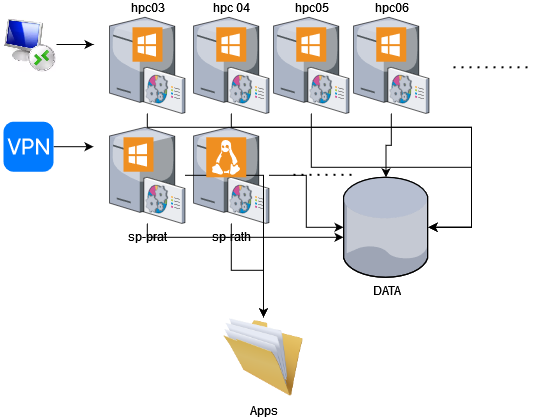
\includegraphics[width=\linewidth,height=0.4\textheight,keepaspectratio]{img/offre-hpc-genes.drawio.png}
\end{column}
\end{columns}

\begin{block}{}
\phantomsection\label{section}
😡 Allocation/partage des ressources

😡 Gestion des packages (r, python\ldots)

😡 Gestion des mise à jour (serveur/application)

😑 Performances

😑 \ldots«~je veux faire du LLM~»

😑 Reproductibilité / Science Ouverte
\end{block}
\end{frame}

\begin{frame}{Nouvelle solution}
\phantomsection\label{nouvelle-solution}
\begin{itemize}
\tightlist
\item
  Moins couteuse pour l'exploitation
\item
  Proposant une meilleure allocation des ressources et leur partage
\item
  Favorisant la reproductibilité
\item
  Favorisant les bonnes pratiques de séparation code/data/traitement
\end{itemize}

➡️


\includegraphics[width=\linewidth,height=0.5\textheight,keepaspectratio]{img/kube-git-s3-transparent.png}
\end{frame}

\begin{frame}{Mais}
\phantomsection\label{mais}
\textbf{Comment embarquer les utilisateurs ?}


\includegraphics[width=\linewidth,height=0.5\textheight,keepaspectratio]{img/chercheur-perplexe-transparent.png}
\end{frame}

\section{La plateforme Onyxia}\label{la-plateforme-onyxia}

\begin{frame}{Onyxia}
\phantomsection\label{onyxia}
\includegraphics[width=\linewidth,height=0.2\textheight,keepaspectratio]{img/logoOnyxia.png}

\textbf{Un cloud opensource pour la datascience} (By Insee)

\begin{block}{}
\phantomsection\label{section-1}
\begin{itemize}
\tightlist
\item
  Pas d'enfermement dans une solution
\item
  Cloud Native
\item
  100\% Open Source (MIT)
\item
  Déploiement facile
\end{itemize}
\end{block}
\end{frame}

\begin{frame}{Onyxia, c'est quoi ?}
\phantomsection\label{onyxia-cest-quoi}
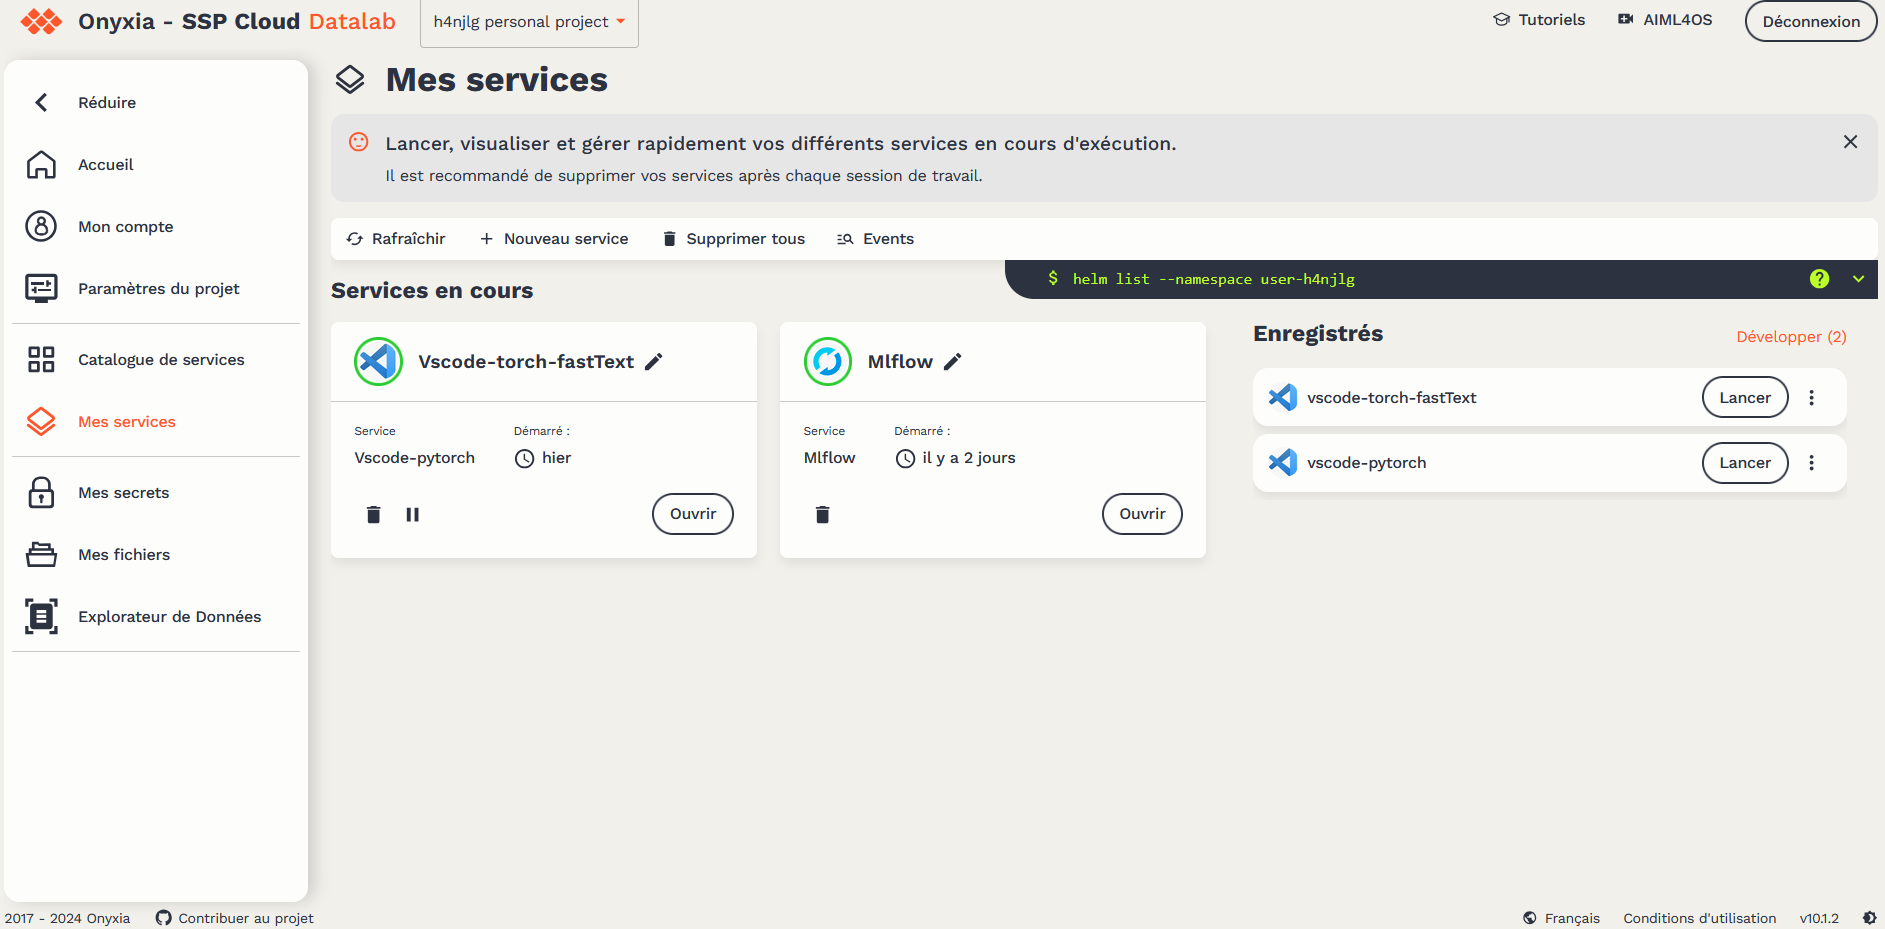
\includegraphics[width=\linewidth,height=0.7\textheight,keepaspectratio]{img/interface-onyxia.png}

\begin{itemize}
\tightlist
\item
  Une application web permettant le déploiement de service sur cluster
  kubernetes
\item
  Un catalogue de services spécialement construit pour l'intégration de
  services externes (Stockage Objet, Gestion de secrets, Git\ldots)
\end{itemize}
\end{frame}

\begin{frame}{Démo}
\phantomsection\label{duxe9mo}
\embedvideo{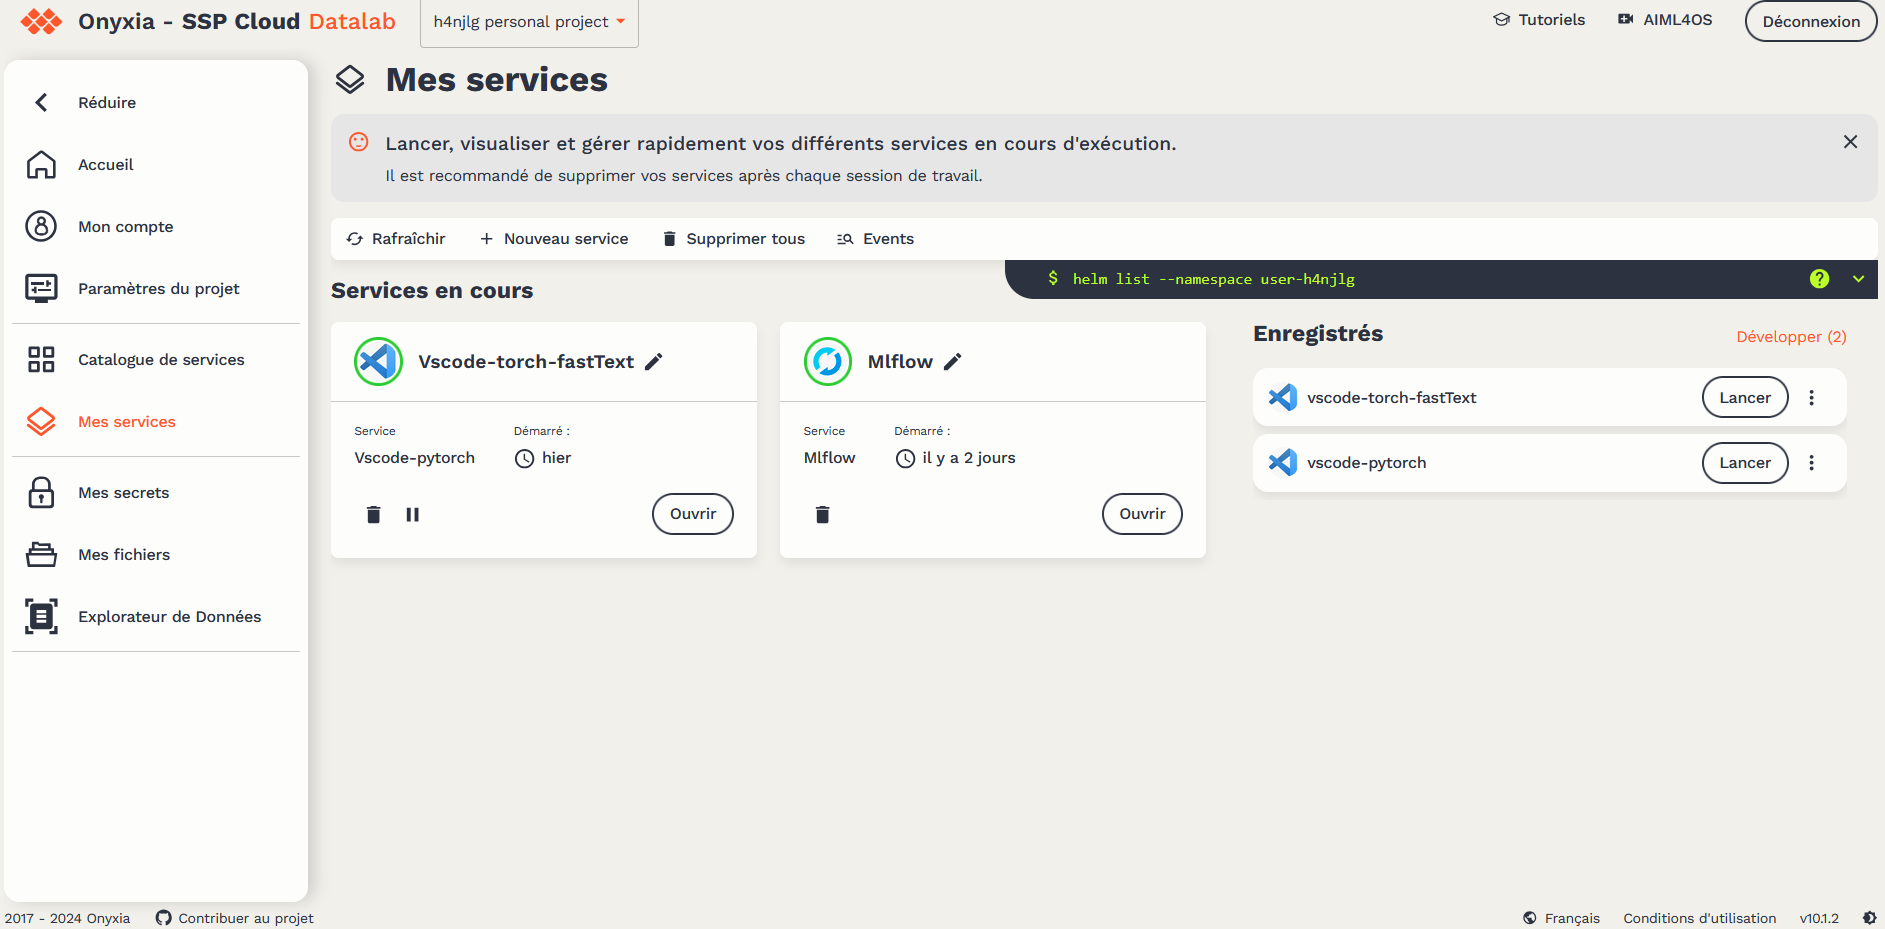
\includegraphics[page=1]{img/interface-onyxia.png}{img/test.mp4}
\end{frame}

\section{L'instance SSPCLOUD}\label{linstance-sspcloud}

\section{Installation et utilisation d'Onyxia au
GENES}\label{installation-et-utilisation-donyxia-au-genes}

\begin{frame}[fragile]{Listings}
\phantomsection\label{listings}
Listings out of the block.

\begin{lstlisting}[language=sh]
#!/bin/bash
echo "Hello world!"
echo "line"
\end{lstlisting}

\begin{block}{Listings in the block.}
\phantomsection\label{listings-in-the-block.}
\begin{lstlisting}[language=sh]
#!/bin/bash
echo "Hello world!"
echo "line"
\end{lstlisting}
\end{block}
\end{frame}

\begin{frame}{Table}
\phantomsection\label{table}
\begin{longtable}[]{@{}lrc@{}}
\toprule\noalign{}
\textbf{Item} & \textbf{Description} & \textbf{Q-ty} \\
\midrule\noalign{}
\endhead
Item A & Item A description & 2 \\
Item B & Item B description & 5 \\
Item C & N/A & 100 \\
\bottomrule\noalign{}
\end{longtable}
\end{frame}

\begin{frame}[fragile]{Single picture}
\phantomsection\label{single-picture}
This is how we insert picture. Caption is produced automatically from
the alt text.

\begin{lstlisting}
![Aleph 0](img/aleph0.png) 
\end{lstlisting}

\begin{figure}
\centering
\pandocbounded{\includegraphics[keepaspectratio]{img/aleph0.png}}
\caption{Aleph 0}
\end{figure}
\end{frame}

\begin{frame}[fragile]{Two or more pictures in a raw}
\phantomsection\label{two-or-more-pictures-in-a-raw}
Here are two pictures in the raw. We can also change two pictures size
(height or width).

\begin{block}{}
\phantomsection\label{section-2}
\begin{lstlisting}
![](img/aleph0.png){height=10%}\ ![](img/aleph0.png){height=30%} 
\end{lstlisting}

\includegraphics[width=\linewidth,height=0.1\textheight,keepaspectratio]{img/aleph0.png}~\includegraphics[width=\linewidth,height=0.3\textheight,keepaspectratio]{img/aleph0.png}
\end{block}
\end{frame}

\begin{frame}{Lists}
\phantomsection\label{lists}
\begin{enumerate}
\tightlist
\item
  Idea 1
\item
  Idea 2

  \begin{itemize}
  \tightlist
  \item
    genius idea A
  \item
    more genius 2
  \end{itemize}
\item
  Conclusion
\end{enumerate}
\end{frame}

\begin{frame}{Two columns of equal width}
\phantomsection\label{two-columns-of-equal-width}
\begin{columns}[T]
\begin{column}{0.48\linewidth}
Left column text.

Another text line.
\end{column}

\begin{column}{0.48\linewidth}
\begin{itemize}
\tightlist
\item
  Item 1.
\item
  Item 2.
\item
  Item 3.
\end{itemize}
\end{column}
\end{columns}
\end{frame}

\begin{frame}{Two columns of with 40:60 split}
\phantomsection\label{two-columns-of-with-4060-split}
\begin{columns}[T]
\begin{column}{0.4\linewidth}
Left column text.

Another text line.
\end{column}

\begin{column}{0.6\linewidth}
\begin{itemize}
\tightlist
\item
  Item 1.
\item
  Item 2.
\item
  Item 3.
\end{itemize}
\end{column}
\end{columns}
\end{frame}

\begin{frame}{Three columns with equal split}
\phantomsection\label{three-columns-with-equal-split}
\begin{columns}[T]
\begin{column}{0.48\linewidth}
Left column text.

Another text line.
\end{column}

\begin{column}{0.48\linewidth}
Middle column list:

\begin{enumerate}
\tightlist
\item
  Item 1.
\item
  Item 2.
\end{enumerate}
\end{column}

\begin{column}{0.48\linewidth}
Right column list:

\begin{itemize}
\tightlist
\item
  Item 1.
\item
  Item 2.
\end{itemize}
\end{column}
\end{columns}
\end{frame}

\begin{frame}{Three columns with 30:40:30 split}
\phantomsection\label{three-columns-with-304030-split}
\begin{columns}[T]
\begin{column}{0.3\linewidth}
Left column text.

Another text line.
\end{column}

\begin{column}{0.4\linewidth}
Middle column list:

\begin{enumerate}
\tightlist
\item
  Item 1.
\item
  Item 2.
\end{enumerate}
\end{column}

\begin{column}{0.3\linewidth}
Right column list:

\begin{itemize}
\tightlist
\item
  Item 1.
\item
  Item 2.
\end{itemize}
\end{column}
\end{columns}
\end{frame}

\begin{frame}{Two columns: image and text}
\phantomsection\label{two-columns-image-and-text}
\begin{columns}[T]
\begin{column}{0.48\linewidth}
\includegraphics[width=\linewidth,height=0.5\textheight,keepaspectratio]{img/aleph0.png}
\end{column}

\begin{column}{0.48\linewidth}
Text in the right column.

List from the right column:

\begin{itemize}
\tightlist
\item
  Item 1.
\item
  Item 2.
\end{itemize}
\end{column}
\end{columns}
\end{frame}

\begin{frame}{Two columns: image and table}
\phantomsection\label{two-columns-image-and-table}
\begin{columns}[T]
\begin{column}{0.48\linewidth}
\includegraphics[width=\linewidth,height=0.5\textheight,keepaspectratio]{img/aleph0.png}
\end{column}

\begin{column}{0.48\linewidth}
\begin{longtable}[]{@{}lc@{}}
\toprule\noalign{}
\textbf{Item} & \textbf{Option} \\
\midrule\noalign{}
\endhead
Item 1 & Option 1 \\
Item 2 & Option 2 \\
\bottomrule\noalign{}
\end{longtable}
\end{column}
\end{columns}
\end{frame}

\begin{frame}{Fancy layout}
\phantomsection\label{fancy-layout}
\begin{block}{Proposal}
\phantomsection\label{proposal}
\begin{itemize}
\tightlist
\item
  Point A
\item
  Point B
\end{itemize}
\end{block}

\begin{columns}[T]
\begin{column}{0.48\linewidth}
\begin{block}{Pros}
\phantomsection\label{pros}
\begin{itemize}
\tightlist
\item
  Good
\item
  Better
\item
  Best
\end{itemize}
\end{block}
\end{column}

\begin{column}{0.48\linewidth}
\begin{block}{Cons}
\phantomsection\label{cons}
\begin{itemize}
\tightlist
\item
  Bad
\item
  Worse
\item
  Worst
\end{itemize}
\end{block}
\end{column}
\end{columns}

\begin{block}{Conclusion}
\phantomsection\label{conclusion}
\begin{itemize}
\tightlist
\item
  Let's go for it!
\item
  No way we go for it!
\end{itemize}
\end{block}
\end{frame}

\end{document}
